\documentclass[a4paper,12pt,oneside,notitlepage,onecolumn]{article}

\usepackage{ucs}
\usepackage[utf8x]{inputenc}

\usepackage{fontenc}
\usepackage{graphicx}

\usepackage[OT4]{fontenc}
\usepackage[polish]{babel}
\usepackage{polski}
\usepackage{indentfirst}
\usepackage{graphics}

\usepackage[dvips]{hyperref}

\author{Michał Bobowski, Andrzej Dudziec}
\date{2013-03-16}
\title{Wektorowa filtracja medianowa - dokumentacja}

\begin{document}
  \maketitle
\section{Usuwanie szumu z obrazów}
Typowe metody akwizycji obrazów (np. matryca Bayera w aparacie fotograficznym) nie są odporne na pojawiające się losowo zakłócenia.
Implikuje to konieczność opracowywania algorytmów filtracji dolnoprzepustowej, czyli 'odszumiania' obrazów.

Najprostsze filtry opierające się na operacji splotu przestrzennego (konwolucji) posiadają znaczącą wadę, objawiającą się w rozmywaniu krawędzi obiektów występujących w obrazie.
Przyczyną tego zjawiska jest fakt, że natura szumu i krawędzi jest do siebie bardzo zbliżona – są to gwałtowne zmiany wartości pikseli, reprezentowane w widmie Fouriera jako składowe wysokoczęstotliwościowe.
Filtracja medianowa jest prostym sposobem na usunięcie szumu z obrazu, bez znaczącego obniżenia jakości krawędzi.
Dla każdego piksela wykonywane jest sortowanie wartości pikseli z sąsiedztwa, a element środkowy tego zbioru staje się nową wartością dla rozpatrywanych współrzędnych.

\section{Wektorowa filtracja medianowa}
Wektorowa filtracja medianowa jest rozwinięciem najprostszej wersji filtru dla obrazów barwnych.
Pikselem wstawianym do obrazu wynikowego nie jest w tym przypadku środkowy element okna analizy, ale piksel najmniej odległy od pozostałych.

Sąsiedztwo pomiędzy punktami może być zdefiniowane na różne sposoby. 
W naszej aplikacji zastosowaliśmy sąsiedztwo euklidesowe, czyli pierwiastek z sumy kwadratów różnic poszczególnych składowych.

\section{Adaptacyjna filtracja medianowa}
Pomimo stosunkowo niewielkich zniekształceń krawędzi, filtracja medianowa wprowadza pewną stratę informacji na obszarach nie będących zakłóceniami.
Adaptacyjny filtr medianowy ogranicza działanie filtru jedynie do pikseli, które znacznie różnią się od sąsiadów, a co za tym idzie z dużym prawdopodobieństwem są zakłóceniami.

Szczegółowy opis algorytmu:
\begin{enumerate}
 \item Zrób coś.
 \item A potem coś jeszcze.
 \item I delektuj się wynikiem.
\end{enumerate}


\section{Uogólniona filtracja medianowa}

\section{Wyniki testów i wnioski}
\subsection{Test 1}
Pierwszy obraz testowy przedstawia mocno zniszczoną fotografię.
Niestety rozmiar zakłóceń jest tak duży, że poprawa jakości przy pomocy filtracji medianowej nie przynosi dobrych rezultatów.
Zwiększanie maski odbija się bardzo negatywnie na zawartości informacyjnej obrazu, a filtracja adaptacyjna nie przynosi prawie żadnych rezultatów.

Przykład ten pokazuje, że filtracja medianowa nie radzi sobie z dużymi ubytkami obrazu.
\begin{figure}
\centering
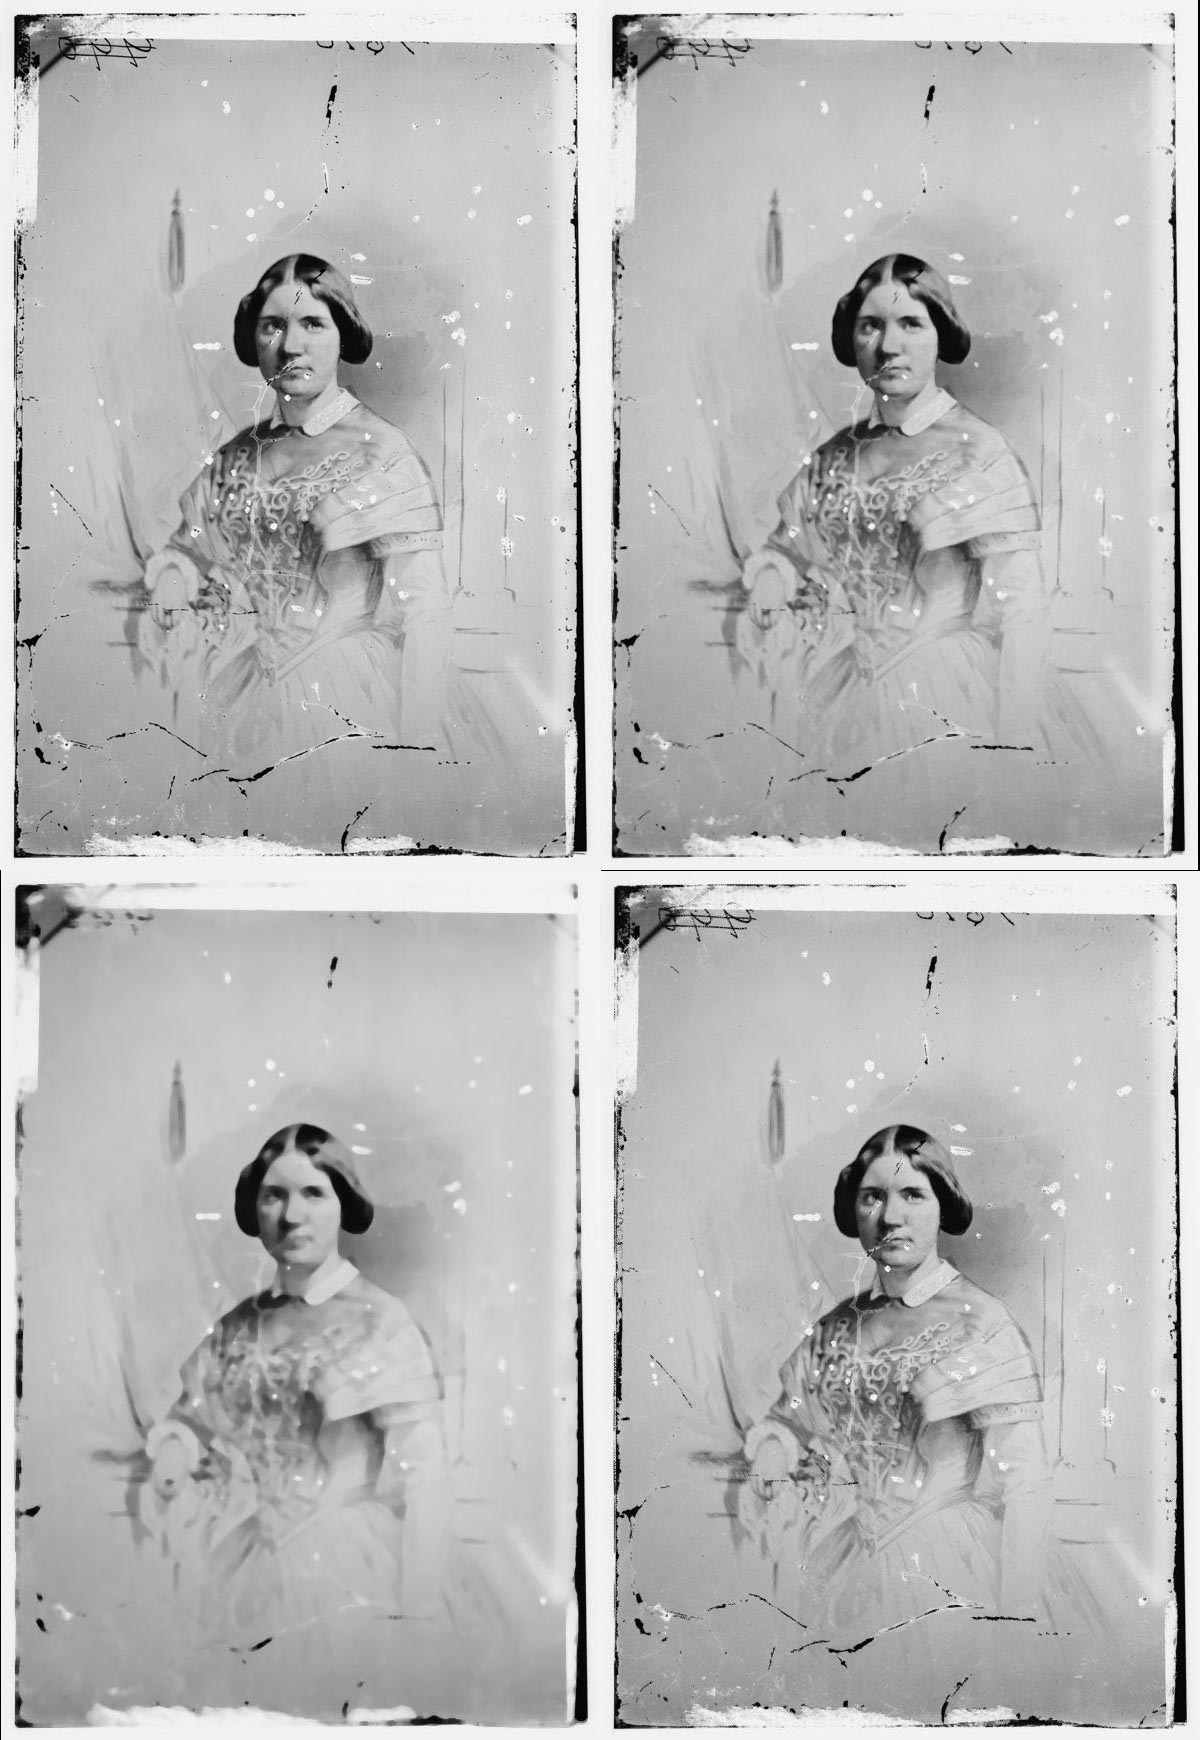
\includegraphics[width=13cm]{test1_final.jpg}
\caption{Od lewej od góry: Oryginał, filtracja 3x3, filtracja 7x7, filtracja adaptacyjna.}
\end{figure}

\subsection{Test 2}
Drugi przykład pokazuje zaszumione zdjęcie góry lodowej.
Wyniki filtracji są znacznie lepsze niż na poprzednim zdjęciu, ponieważ natura szumu jest bardziej korzystna dla rozpatrywanej metody.
Zakłócenia występują punktowo i są od siebie oddalone.

Filtracja oknem 3x3 usuwa praktycznie wszystkie zakłócenia, chociaż powoduje zauważalne rozmycie niektórych szczegółów.
Dobre efekty daje natomiast filtracja adaptacyjna, która usuwa większość zakłóceń, nie obniżając przy tym jakości obrazu.

\begin{figure}
\centering
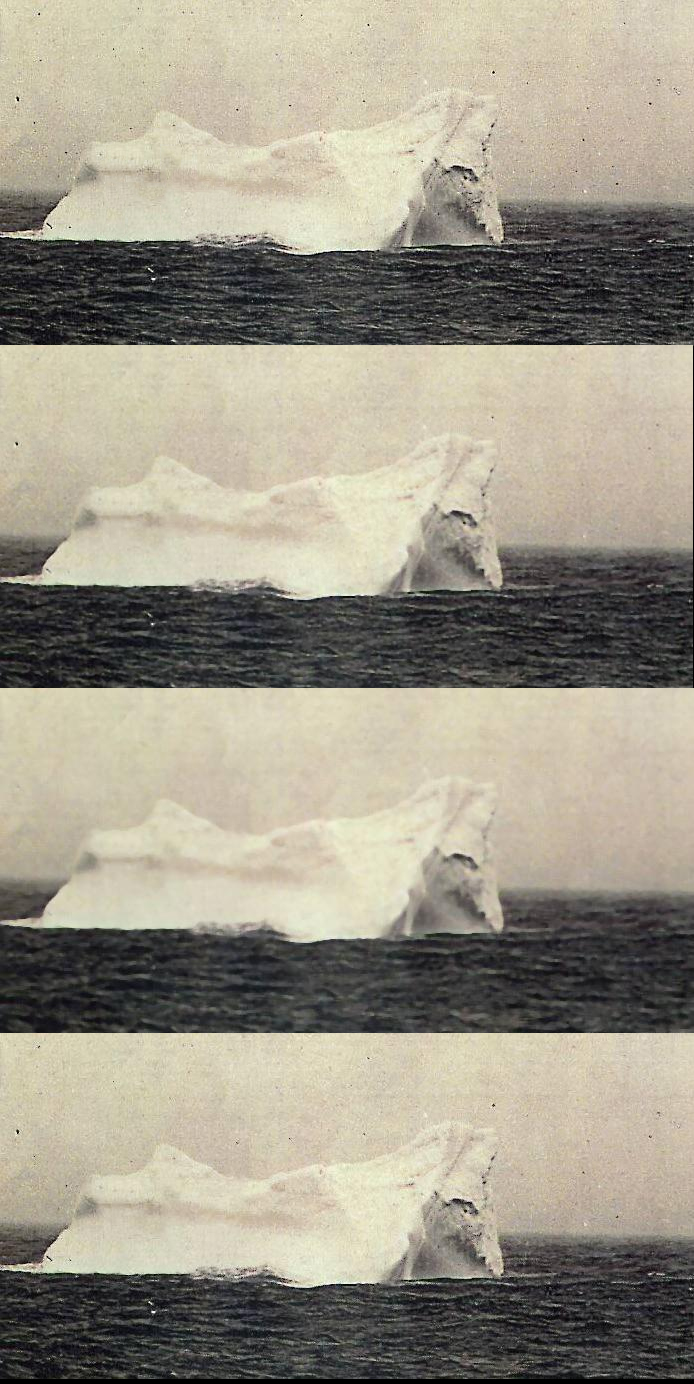
\includegraphics[width=10cm]{test2_final.jpg}
\caption{Od góry: Oryginał, filtracja 3x3, filtracja 5x5, filtracja adaptacyjna.}
\end{figure}

\subsection{Test 3}
Przykład trzeci przedstawia bardzo silnie zaszumiony obraz.
W tym przypadku filtracja medianowa również nie radzi sobie z zakłóceniami, ponieważ obraz praktycznie cały składa się z szumu.
Efekty przynosi dopiero znaczne zwiększenie rozmiaru okna analizy (7x7), co z kolei rozmazuje szczegóły.
\begin{figure}
\centering
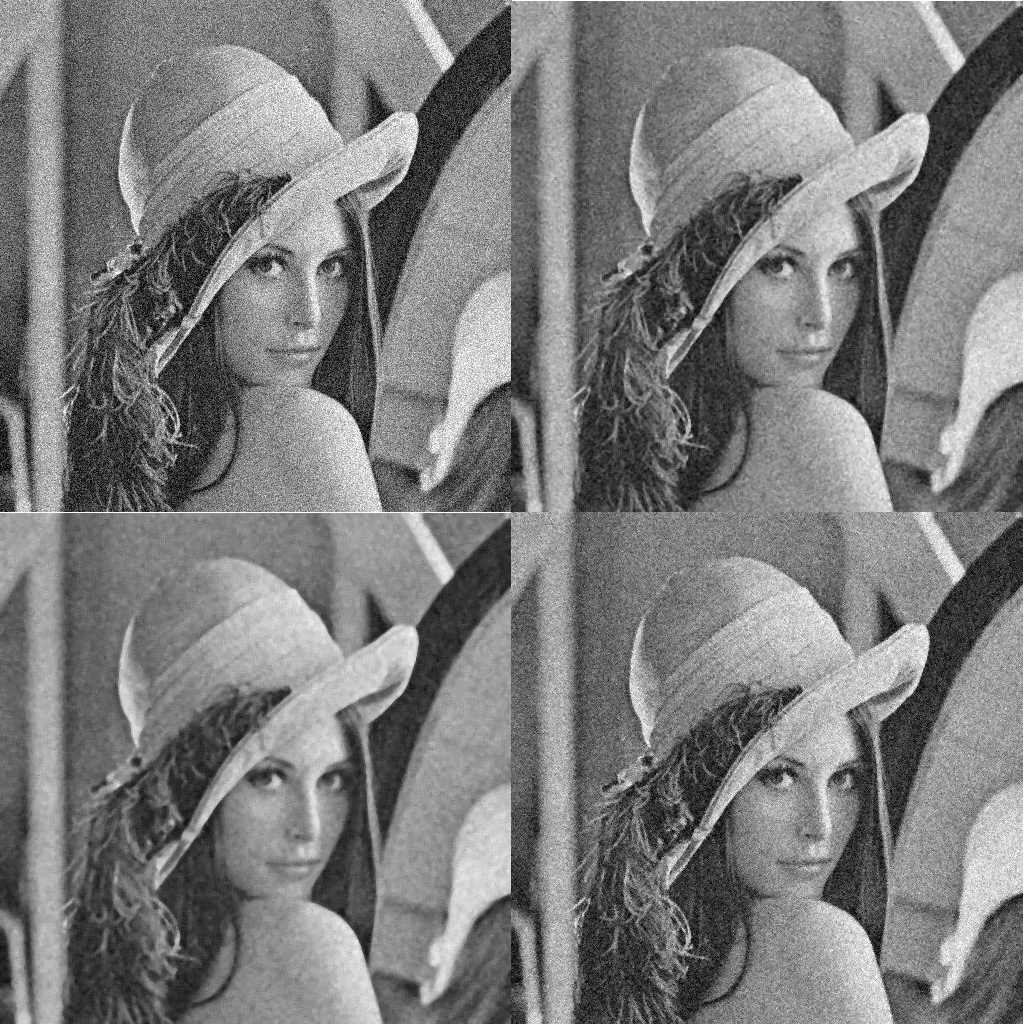
\includegraphics[width=13cm]{test3_final.png}
\caption{Od lewej od góry: Oryginał, filtracja 3x3, filtracja 7x7, filtracja adaptacyjna.}
\end{figure}

\subsection{Test 4}
Czwarty obraz testowy zawiera bardzo rzadkie i punktowe zakłócenia, więc podobnie jak w przypadku obrazu drugiego, efekty filtracji są bardzo dobre.
Łatwo widoczna jest również różnica pomiędzy filtracją zwykłą i adaptacyjną.
\begin{figure}
\centering
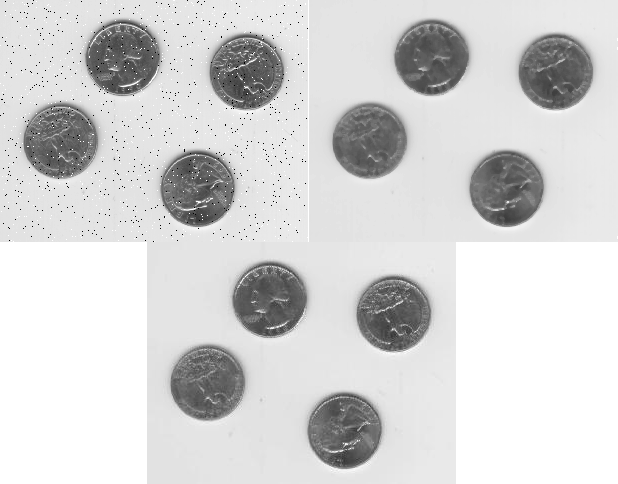
\includegraphics[width=13cm]{test4_final.png}
\caption{Od lewej od góry: Oryginał, filtracja 3x3, filtracja adaptacyjna.}
\end{figure}

\subsection{Test 5}
\begin{figure}
\centering
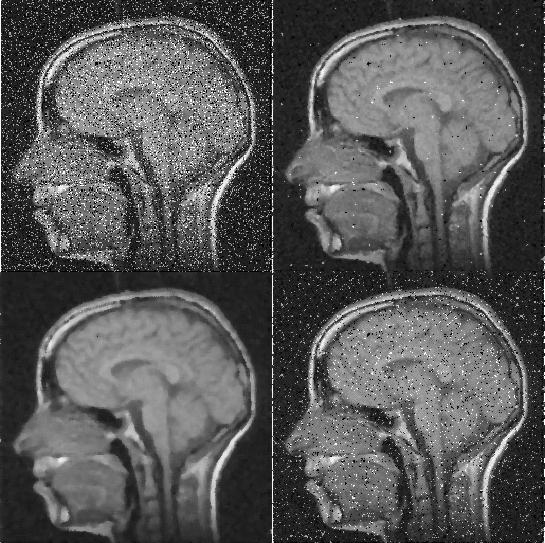
\includegraphics[width=13cm]{test5_final.JPG}
\caption{Od lewej od góry: Oryginał, filtracja 3x3, filtracja 5x5, filtracja adaptacyjna.}
\end{figure}

\end{document}
